%%
% Copyright (c) 2017 - 2019, Pascal Wagler;  
% Copyright (c) 2014 - 2019, John MacFarlane
% 
% All rights reserved.
% 
% Redistribution and use in source and binary forms, with or without 
% modification, are permitted provided that the following conditions 
% are met:
% 
% - Redistributions of source code must retain the above copyright 
% notice, this list of conditions and the following disclaimer.
% 
% - Redistributions in binary form must reproduce the above copyright 
% notice, this list of conditions and the following disclaimer in the 
% documentation and/or other materials provided with the distribution.
% 
% - Neither the name of John MacFarlane nor the names of other 
% contributors may be used to endorse or promote products derived 
% from this software without specific prior written permission.
% 
% THIS SOFTWARE IS PROVIDED BY THE COPYRIGHT HOLDERS AND CONTRIBUTORS 
% "AS IS" AND ANY EXPRESS OR IMPLIED WARRANTIES, INCLUDING, BUT NOT 
% LIMITED TO, THE IMPLIED WARRANTIES OF MERCHANTABILITY AND FITNESS 
% FOR A PARTICULAR PURPOSE ARE DISCLAIMED. IN NO EVENT SHALL THE 
% COPYRIGHT OWNER OR CONTRIBUTORS BE LIABLE FOR ANY DIRECT, INDIRECT, 
% INCIDENTAL, SPECIAL, EXEMPLARY, OR CONSEQUENTIAL DAMAGES (INCLUDING,
% BUT NOT LIMITED TO, PROCUREMENT OF SUBSTITUTE GOODS OR SERVICES; 
% LOSS OF USE, DATA, OR PROFITS; OR BUSINESS INTERRUPTION) HOWEVER 
% CAUSED AND ON ANY THEORY OF LIABILITY, WHETHER IN CONTRACT, STRICT 
% LIABILITY, OR TORT (INCLUDING NEGLIGENCE OR OTHERWISE) ARISING IN 
% ANY WAY OUT OF THE USE OF THIS SOFTWARE, EVEN IF ADVISED OF THE 
% POSSIBILITY OF SUCH DAMAGE.
%%

%%
% This is the Eisvogel pandoc LaTeX template.
%
% For usage information and examples visit the official GitHub page:
% https://github.com/Wandmalfarbe/pandoc-latex-template
%%

\PassOptionsToPackage{unicode=true}{hyperref} % options for packages loaded elsewhere
\PassOptionsToPackage{hyphens}{url}
\PassOptionsToPackage{dvipsnames,svgnames*,x11names*,table}{xcolor}
%
\documentclass[
  10pt,
  english,
  letterpaper,
,tablecaptionabove
]{scrartcl}
\usepackage{lmodern}
\usepackage{setspace}
\setstretch{1.2}
\usepackage{amssymb,amsmath}
\usepackage{ifxetex,ifluatex}
\ifnum 0\ifxetex 1\fi\ifluatex 1\fi=0 % if pdftex
  \usepackage[T1]{fontenc}
  \usepackage[utf8]{inputenc}
  \usepackage{textcomp} % provides euro and other symbols
\else % if luatex or xelatex
  \usepackage{unicode-math}
  \defaultfontfeatures{Scale=MatchLowercase}
  \defaultfontfeatures[\rmfamily]{Ligatures=TeX,Scale=1}
\fi
% use upquote if available, for straight quotes in verbatim environments
\IfFileExists{upquote.sty}{\usepackage{upquote}}{}
\IfFileExists{microtype.sty}{% use microtype if available
  \usepackage[]{microtype}
  \UseMicrotypeSet[protrusion]{basicmath} % disable protrusion for tt fonts
}{}
\makeatletter
\@ifundefined{KOMAClassName}{% if non-KOMA class
  \IfFileExists{parskip.sty}{%
    \usepackage{parskip}
  }{% else
    \setlength{\parindent}{0pt}
    \setlength{\parskip}{6pt plus 2pt minus 1pt}}
}{% if KOMA class
  \KOMAoptions{parskip=half}}
\makeatother
\usepackage{xcolor}
\definecolor{default-linkcolor}{HTML}{A50000}
\definecolor{default-filecolor}{HTML}{A50000}
\definecolor{default-citecolor}{HTML}{4077C0}
\definecolor{default-urlcolor}{HTML}{4077C0}
\IfFileExists{xurl.sty}{\usepackage{xurl}}{} % add URL line breaks if available
\IfFileExists{bookmark.sty}{\usepackage{bookmark}}{\usepackage{hyperref}}
\hypersetup{
  pdftitle={Priority Queues and Binary Heaps (Part 2)},
  pdfauthor={Connor Baker},
  pdfsubject={Heaps},
  pdfkeywords={Lecture, Priority Queues, Binary Heaps},
  pdfborder={0 0 0},
  breaklinks=true}
\urlstyle{same}  % don't use monospace font for urls
\usepackage[margin=2.5cm,includehead=true,includefoot=true,centering]{geometry}
\usepackage{listings}
\newcommand{\passthrough}[1]{#1}
\lstset{defaultdialect=[5.3]Lua}
\lstset{defaultdialect=[x86masm]Assembler}
\usepackage{graphicx,grffile}
\makeatletter
\def\maxwidth{\ifdim\Gin@nat@width>\linewidth\linewidth\else\Gin@nat@width\fi}
\def\maxheight{\ifdim\Gin@nat@height>\textheight\textheight\else\Gin@nat@height\fi}
\makeatother
% Scale images if necessary, so that they will not overflow the page
% margins by default, and it is still possible to overwrite the defaults
% using explicit options in \includegraphics[width, height, ...]{}
\setkeys{Gin}{width=\maxwidth,height=\maxheight,keepaspectratio}
\setlength{\emergencystretch}{3em}  % prevent overfull lines
\providecommand{\tightlist}{%
  \setlength{\itemsep}{0pt}\setlength{\parskip}{0pt}}
\setcounter{secnumdepth}{-\maxdimen} % remove section numbering
% Redefines (sub)paragraphs to behave more like sections
\ifx\paragraph\undefined\else
  \let\oldparagraph\paragraph
  \renewcommand{\paragraph}[1]{\oldparagraph{#1}\mbox{}}
\fi
\ifx\subparagraph\undefined\else
  \let\oldsubparagraph\subparagraph
  \renewcommand{\subparagraph}[1]{\oldsubparagraph{#1}\mbox{}}
\fi

% Make use of float-package and set default placement for figures to H
\usepackage{float}
\floatplacement{figure}{H}

\setcounter{page}{0}
\lstset{breaklines=true}
\lstset{postbreak=\raisebox{0ex}[0ex][0ex]{\ensuremath{\color{blue}\hookrightarrow\space}}}
\usepackage{datetime}
\settimeformat{ampmtime}
\usepackage{lastpage}
\ifnum 0\ifxetex 1\fi=0 % if pdftex or luatex
  \usepackage[shorthands=off,main=english]{babel}
\else % if xetex
    % See issue https://github.com/reutenauer/polyglossia/issues/127
  \renewcommand*\familydefault{\sfdefault}
    % load polyglossia as late as possible as it *could* call bidi if RTL lang (e.g. Hebrew or Arabic)
  \usepackage{polyglossia}
  \setmainlanguage[]{english}
\fi

\title{Priority Queues and Binary Heaps (Part 2)}
\usepackage{etoolbox}
\makeatletter
\providecommand{\subtitle}[1]{% add subtitle to \maketitle
  \apptocmd{\@title}{\par {\large #1 \par}}{}{}
}
\makeatother
\subtitle{Heap sorting, creation of heaps, and heap creation complexity}
\author{Connor Baker}
\date{2019-04-04, Compiled on \today~at \currenttime}





%%
%% added
%%

%
% language specification
%
% If no language is specified, use English as the default main document language.
%


%
% for the background color of the title page
%
\usepackage{pagecolor}
\usepackage{afterpage}

%
% TOC depth and 
% section numbering depth
%
\setcounter{tocdepth}{3}

%
% break urls
%
\PassOptionsToPackage{hyphens}{url}

%
% When using babel or polyglossia with biblatex, loading csquotes is recommended 
% to ensure that quoted texts are typeset according to the rules of your main language.
%
\usepackage{csquotes}

%
% captions
%
\definecolor{caption-color}{HTML}{777777}
\usepackage[font={stretch=1.2}, textfont={color=caption-color}, position=top, skip=4mm, labelfont=bf, singlelinecheck=false, justification=raggedright]{caption}
\setcapindent{0em}

%
% blockquote
%
\definecolor{blockquote-border}{RGB}{221,221,221}
\definecolor{blockquote-text}{RGB}{119,119,119}
\usepackage{mdframed}
\newmdenv[rightline=false,bottomline=false,topline=false,linewidth=3pt,linecolor=blockquote-border,skipabove=\parskip]{customblockquote}
\renewenvironment{quote}{\begin{customblockquote}\list{}{\rightmargin=0em\leftmargin=0em}%
\item\relax\color{blockquote-text}\ignorespaces}{\unskip\unskip\endlist\end{customblockquote}}

%
% Source Sans Pro as the de­fault font fam­ily
% Source Code Pro for monospace text
%
% 'default' option sets the default 
% font family to Source Sans Pro, not \sfdefault.
%
\usepackage[default]{sourcesanspro}
\usepackage{sourcecodepro}

% XeLaTeX specific adjustments for straight quotes: https://tex.stackexchange.com/a/354887
% This issue is already fixed (see https://github.com/silkeh/latex-sourcecodepro/pull/5) but the 
% fix is still unreleased.
% TODO: Remove this workaround when the new version of sourcecodepro is released on CTAN.
\ifxetex
\makeatletter
\defaultfontfeatures[\ttfamily]
  { Numbers   = \sourcecodepro@figurestyle,
    Scale     = \SourceCodePro@scale,
    Extension = .otf }
\setmonofont
  [ UprightFont    = *-\sourcecodepro@regstyle,
    ItalicFont     = *-\sourcecodepro@regstyle It,
    BoldFont       = *-\sourcecodepro@boldstyle,
    BoldItalicFont = *-\sourcecodepro@boldstyle It ]
  {SourceCodePro}
\makeatother
\fi

%
% heading color
%
\definecolor{heading-color}{RGB}{40,40,40}
\addtokomafont{section}{\color{heading-color}}
% When using the classes report, scrreprt, book, 
% scrbook or memoir, uncomment the following line.
%\addtokomafont{chapter}{\color{heading-color}}

%
% variables for title and author
%
\usepackage{titling}
\title{Priority Queues and Binary Heaps (Part 2)}
\author{Connor Baker}

%
% tables
%

%
% remove paragraph indention
%
\setlength{\parindent}{0pt}
\setlength{\parskip}{6pt plus 2pt minus 1pt}
\setlength{\emergencystretch}{3em}  % prevent overfull lines

%
%
% Listings
%
%


%
% listing colors
%
\definecolor{listing-background}{HTML}{F7F7F7}
\definecolor{listing-rule}{HTML}{B3B2B3}
\definecolor{listing-numbers}{HTML}{B3B2B3}
\definecolor{listing-text-color}{HTML}{000000}
\definecolor{listing-keyword}{HTML}{435489}
\definecolor{listing-identifier}{HTML}{435489}
\definecolor{listing-string}{HTML}{00999A}
\definecolor{listing-comment}{HTML}{8E8E8E}
\definecolor{listing-javadoc-comment}{HTML}{006CA9}

\lstdefinestyle{eisvogel_listing_style}{
  language         = java,
  numbers          = left,
  xleftmargin      = 2.7em,
  framexleftmargin = 2.5em,
  backgroundcolor  = \color{listing-background},
  basicstyle       = \color{listing-text-color}\small\ttfamily{}\linespread{1.15}, % print whole listing small
  breaklines       = true,
  frame            = single,
  framesep         = 0.19em,
  rulecolor        = \color{listing-rule},
  frameround       = ffff,
  tabsize          = 4,
  numberstyle      = \color{listing-numbers},
  aboveskip        = -0.7em,
  belowskip        = 0.1em,
  abovecaptionskip = 0em,
  belowcaptionskip = 1em,
  keywordstyle     = \color{listing-keyword}\bfseries,
  classoffset      = 0,
  sensitive        = true,
  identifierstyle  = \color{listing-identifier},
  commentstyle     = \color{listing-comment},
  morecomment      = [s][\color{listing-javadoc-comment}]{/**}{*/},
  stringstyle      = \color{listing-string},
  showstringspaces = false,
  escapeinside     = {/*@}{@*/}, % Allow LaTeX inside these special comments
  literate         =
  {á}{{\'a}}1 {é}{{\'e}}1 {í}{{\'i}}1 {ó}{{\'o}}1 {ú}{{\'u}}1
  {Á}{{\'A}}1 {É}{{\'E}}1 {Í}{{\'I}}1 {Ó}{{\'O}}1 {Ú}{{\'U}}1
  {à}{{\`a}}1 {è}{{\'e}}1 {ì}{{\`i}}1 {ò}{{\`o}}1 {ù}{{\`u}}1
  {À}{{\`A}}1 {È}{{\'E}}1 {Ì}{{\`I}}1 {Ò}{{\`O}}1 {Ù}{{\`U}}1
  {ä}{{\"a}}1 {ë}{{\"e}}1 {ï}{{\"i}}1 {ö}{{\"o}}1 {ü}{{\"u}}1
  {Ä}{{\"A}}1 {Ë}{{\"E}}1 {Ï}{{\"I}}1 {Ö}{{\"O}}1 {Ü}{{\"U}}1
  {â}{{\^a}}1 {ê}{{\^e}}1 {î}{{\^i}}1 {ô}{{\^o}}1 {û}{{\^u}}1
  {Â}{{\^A}}1 {Ê}{{\^E}}1 {Î}{{\^I}}1 {Ô}{{\^O}}1 {Û}{{\^U}}1
  {œ}{{\oe}}1 {Œ}{{\OE}}1 {æ}{{\ae}}1 {Æ}{{\AE}}1 {ß}{{\ss}}1
  {ç}{{\c c}}1 {Ç}{{\c C}}1 {ø}{{\o}}1 {å}{{\r a}}1 {Å}{{\r A}}1
  {€}{{\EUR}}1 {£}{{\pounds}}1 {«}{{\guillemotleft}}1
  {»}{{\guillemotright}}1 {ñ}{{\~n}}1 {Ñ}{{\~N}}1 {¿}{{?`}}1
  {…}{{\ldots}}1 {≥}{{>=}}1 {≤}{{<=}}1 {„}{{\glqq}}1 {“}{{\grqq}}1
  {”}{{''}}1
}
\lstset{style=eisvogel_listing_style}

\lstdefinelanguage{XML}{
  morestring      = [b]",
  moredelim       = [s][\bfseries\color{listing-keyword}]{<}{\ },
  moredelim       = [s][\bfseries\color{listing-keyword}]{</}{>},
  moredelim       = [l][\bfseries\color{listing-keyword}]{/>},
  moredelim       = [l][\bfseries\color{listing-keyword}]{>},
  morecomment     = [s]{<?}{?>},
  morecomment     = [s]{<!--}{-->},
  commentstyle    = \color{listing-comment},
  stringstyle     = \color{listing-string},
  identifierstyle = \color{listing-identifier}
}

%
% header and footer
%
\usepackage{fancyhdr}

\fancypagestyle{eisvogel-header-footer}{
  \fancyhead{}
  \fancyfoot{}
  \lhead[2019-04-04]{Priority Queues and Binary Heaps (Part 2)}
  \chead[]{}
  \rhead[Priority Queues and Binary Heaps (Part 2)]{2019-04-04}
  \lfoot[\thepage~of \pageref{LastPage}]{Connor Baker}
  \cfoot[]{}
  \rfoot[Connor Baker]{\thepage~of \pageref{LastPage}}
  \renewcommand{\headrulewidth}{0.4pt}
  \renewcommand{\footrulewidth}{0.4pt}
}
\pagestyle{eisvogel-header-footer}

%%
%% end added
%%

\begin{document}

%%
%% begin titlepage
%%

\begin{titlepage}
\newgeometry{left=6cm}
\definecolor{titlepage-color}{HTML}{FFFFFF}
\newpagecolor{titlepage-color}\afterpage{\restorepagecolor}
\newcommand{\colorRule}[3][black]{\textcolor[HTML]{#1}{\rule{#2}{#3}}}
\begin{flushleft}
\noindent
\\[-1em]
\color[HTML]{0d47a1}
\makebox[0pt][l]{\colorRule[0d47a1]{1.3\textwidth}{2pt}}
\par
\noindent

{ \setstretch{1.4}
\vfill
\noindent {\huge \textbf{\textsf{Priority Queues and Binary Heaps (Part 2)}}}
\vskip 1em
{\Large \textsf{Heap sorting, creation of heaps, and heap creation complexity}}
\vskip 2em
\noindent
{\Large \textsf{Connor Baker}
\vfill
}


\textsf{2019-04-04, Compiled on \today~at \currenttime}}
\end{flushleft}
\end{titlepage}
\restoregeometry

%%
%% end titlepage
%%



\hypertarget{priority-queues-and-binary-heaps-part-2}{%
\section{Priority Queues and Binary Heaps (Part
2)}\label{priority-queues-and-binary-heaps-part-2}}

\hypertarget{heaps-for-sorting}{%
\subsection{Heaps for Sorting}\label{heaps-for-sorting}}

\begin{itemize}
\tightlist
\item
  How would you use a priority queue or a heap to sort a collection of
  values?

  \begin{itemize}
  \tightlist
  \item
    Max heap: Sort in descending order
  \item
    Min heap: Sort in ascending order
  \end{itemize}
\item
  Steps: insert and delete

  \begin{itemize}
  \tightlist
  \item
    First, insert each value into the heap
  \item
    Then, remove each value one-by-one until none remain
  \end{itemize}
\end{itemize}

\hypertarget{out-of-place-heap-sort-issues}{%
\subsection{Out-Of-Place Heap Sort:
Issues}\label{out-of-place-heap-sort-issues}}

\begin{itemize}
\tightlist
\item
  Data duplication is required

  \begin{itemize}
  \tightlist
  \item
    We need to create a copy of the original data set, store it in a
    priority queue, and then copy it back

    \begin{itemize}
    \tightlist
    \item
      This doubles the memory requirement
    \end{itemize}
  \end{itemize}
\item
  For large data sets, this duplication hurts

  \begin{itemize}
  \tightlist
  \item
    We ideally want an approach to perform in-place sorting
  \end{itemize}
\end{itemize}

\hypertarget{in-place-heap-sort}{%
\subsection{In-Place Heap Sort}\label{in-place-heap-sort}}

\begin{itemize}
\tightlist
\item
  Task: given a non-heap array, sort it using the ideas that we've seen
  used to make heap-sort work
\item
  Three main issues:

  \begin{enumerate}
  \def\labelenumi{\arabic{enumi}.}
  \tightlist
  \item
    The array is full with some value at index 0

    \begin{itemize}
    \tightlist
    \item
      Our heap has a dummy 0-index item
    \end{itemize}
  \item
    Where do we store the value we delete from the heap?
  \item
    How do we make the non-heap array a heap?
  \end{enumerate}
\end{itemize}

\hypertarget{issue-1-changed-root-location}{%
\subsection{Issue 1: Changed Root
Location}\label{issue-1-changed-root-location}}

\begin{itemize}
\tightlist
\item
  Root at 1

  \begin{itemize}
  \tightlist
  \item
    \passthrough{\lstinline!static int root() \{ return 1; \}!}
  \item
    \passthrough{\lstinline!static int left(int i) \{ return i * 2; \}!}
  \item
    \passthrough{\lstinline!static int right(int i) \{ return i * 2 + 1; \}!}
  \item
    \passthrough{\lstinline!static int parent(int i) \{ return i / 2; \}!}
  \end{itemize}
\item
  Root at 0

  \begin{itemize}
  \tightlist
  \item
    \passthrough{\lstinline!static int root() \{ return 0; \}!}
  \item
    \passthrough{\lstinline!static int left(int i) \{ return i * 2 + 1; \}!}
  \item
    \passthrough{\lstinline!static int right(int i) \{ return i * 2 + 2; \}!}
  \item
    \passthrough{\lstinline!static int parent(int i) \{ return (i - 1) / 2; \}!}
  \end{itemize}
\end{itemize}

\hypertarget{issue-2-space-reuse}{%
\subsection{Issue 2: Space Reuse}\label{issue-2-space-reuse}}

\begin{itemize}
\tightlist
\item
  If we have a heap already\ldots{}
\item
  Space available for values removed from the heap

  \begin{itemize}
  \tightlist
  \item
    Remove an element from a heap
  \item
    Now there's open space at the end of the array (since the complete
    tree is shrinking, it must first withdraw from that portion of the
    array)
  \item
    Put the removed element at the end of the array
  \item
    Repeat this process until the array is empty
  \end{itemize}
\end{itemize}

\hypertarget{space-reuse-example}{%
\subsection{Space Reuse: Example}\label{space-reuse-example}}

\begin{itemize}
\tightlist
\item
  Images, left to right

  \begin{itemize}
  \tightlist
  \item
    Initial heap

    \begin{itemize}
    \tightlist
    \item
      10 unsorted values
    \end{itemize}
  \item
    After the first \passthrough{\lstinline!deleteMax()!}

    \begin{itemize}
    \tightlist
    \item
      9 unsorted and 1 sorted
    \end{itemize}
  \item
    After the second \passthrough{\lstinline!deleteMax()!}

    \begin{itemize}
    \tightlist
    \item
      8 unsorted and 2 sorted
    \end{itemize}
  \end{itemize}
\end{itemize}

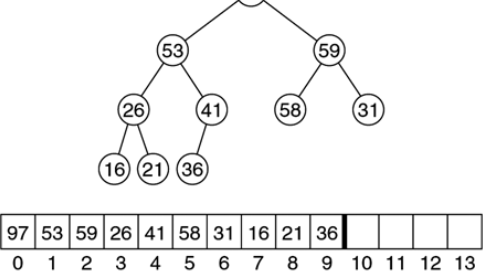
\includegraphics[width=0.33\textwidth,height=\textheight]{images/1.png}
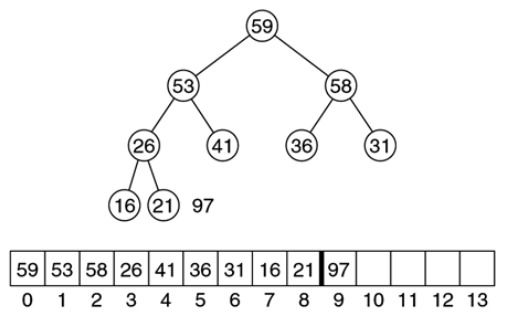
\includegraphics[width=0.33\textwidth,height=\textheight]{images/2.png}
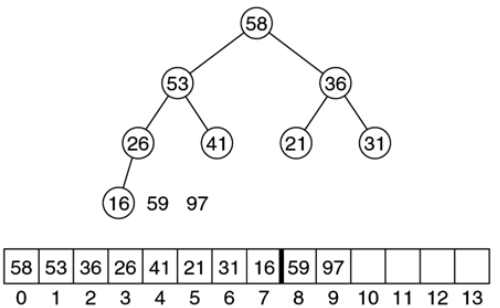
\includegraphics[width=0.33\textwidth,height=\textheight]{images/3.png}

\hypertarget{issue-3-heapify}{%
\subsection{\texorpdfstring{Issue 3:
\enquote{Heapify}}{Issue 3: ``Heapify''}}\label{issue-3-heapify}}

\begin{itemize}
\tightlist
\item
  We need to be able to convert an existing array into a heap
\item
  We can build the heap bottom up through repeated application of
  \passthrough{\lstinline!percolateDown()!}

  \begin{itemize}
  \tightlist
  \item
    Start one level above the bottom
  \item
    Work right to left, bottom up
  \item
    Apply \passthrough{\lstinline!percolateDown()!} for each non-leaf
    node

    \begin{itemize}
    \tightlist
    \item
      Compare the non-leaf node with its children
    \item
      Swap if the heap order is violated
    \end{itemize}
  \end{itemize}
\end{itemize}

\hypertarget{example-min-heap}{%
\subsection{Example: Min Heap}\label{example-min-heap}}

\begin{itemize}
\tightlist
\item
  Note: \passthrough{\lstinline![n]!} represents the index for the value
  \passthrough{\lstinline!n!}
\end{itemize}

\begin{figure}
\centering
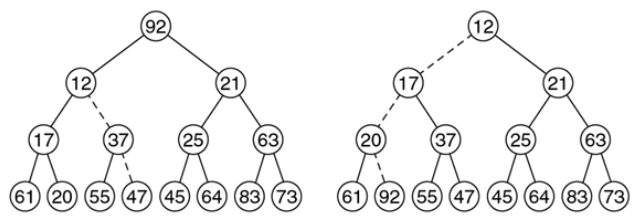
\includegraphics[width=0.75\textwidth,height=\textheight]{images/4.png}
\caption{\passthrough{\lstinline!precolateDown([20])!} and
\passthrough{\lstinline!precolateDown([21])!}}
\end{figure}

\begin{figure}
\centering
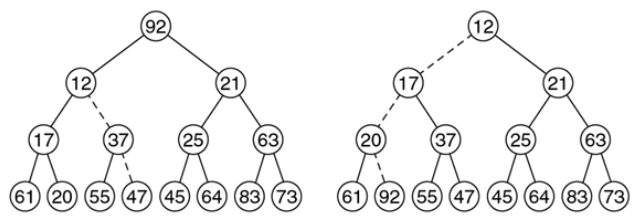
\includegraphics[width=0.75\textwidth,height=\textheight]{images/5.png}
\caption{\passthrough{\lstinline!precolateDown([47])!} and
\passthrough{\lstinline!precolateDown([92])!}}
\end{figure}

\hypertarget{heapify-implementation}{%
\subsection{Heapify Implementation}\label{heapify-implementation}}

\begin{lstlisting}[language=Java]
public void buildHeap() {
  for (int i = parent(this.size); i >= root(); i--) {
    this.percolateDown(i);
  }
}
\end{lstlisting}

\begin{itemize}
\tightlist
\item
  What is the complexity?

  \begin{itemize}
  \tightlist
  \item
    \textbf{Answer}
  \end{itemize}
\item
  How many loop iterations are there?

  \begin{itemize}
  \tightlist
  \item
    \textbf{Answer}
  \end{itemize}
\item
  How many edges do we have to move down for each iteration?

  \begin{itemize}
  \tightlist
  \item
    \textbf{Answer}
  \end{itemize}
\item
  Worst case?

  \begin{itemize}
  \tightlist
  \item
    \textbf{Answer}
  \end{itemize}
\end{itemize}

\hypertarget{heapify-complexity}{%
\subsection{Heapify Complexity}\label{heapify-complexity}}

\begin{itemize}
\tightlist
\item
  Assume the tree height is \(h\), and count the work as the number of
  comparisons/swaps done at each level

  \begin{itemize}
  \tightlist
  \item
    At the bottom (level 0) there are (at most) \(2^h\) nodes

    \begin{itemize}
    \tightlist
    \item
      We do not do anything, so the work is zero
    \end{itemize}
  \item
    Level 1 has \(2^{h-1}\) nodes

    \begin{itemize}
    \tightlist
    \item
      Each might move down (at most) 1 level
    \end{itemize}
  \item
    Level 2 has \(2^{h-2}\) nodes

    \begin{itemize}
    \tightlist
    \item
      Each might move down (at most) 2 levels
    \end{itemize}
  \item
    Level \(i\) is the \(i\)th from the bottom and has \(2^{h-i}\) nodes
  \item
    Level \(h\) is the root, has \(2^{h-h} = 2^0 = 1\) node
  \end{itemize}
\item
  Each level \(i\) node can move at most \(i\) steps down, so
  \[\text{moves} = \sum_{i=1}^h i\times 2^{h-i} = \sum_{i=1}^{\log_2(n)} i\times 2^{\log_2(n-i)} = \sum_{i=1}^{\log_2(n)} i\times \frac{2^{\log_2(n)}}{2^i} = n \sum_{i=1}^{\log_2(n)} \frac{i}{2^i}.\]
  Since \[\sum_{i=1}^\infty \frac{i}{2^i} \rightarrow 2,\] we know that
  \[n \sum_{i=1}^{\log_2(n)} \frac{i}{2^i} \leq n\times 2\] and
  \[n\times 2 \in O(n).\] Therefore \[\text{moves} \in O(n).\]
\end{itemize}

\hypertarget{weiss-theorem}{%
\subsection{Weiss Theorem}\label{weiss-theorem}}

\begin{itemize}
\tightlist
\item
  \emph{Theorem 21.1:} For a perfect tree of height \(h\) with
  \(n = 2^{h+1} - 1\) nodes, the sum of the heights of the nodes is
  \(n-h-1\)

  \begin{itemize}
  \tightlist
  \item
    This is the upper bound for a complete binary tree
  \item
    The sum of the heights is equivalent to the max number of swaps
    required, so it is \(O(n)\)
  \end{itemize}
\item
  We can arrive at the proof by darkening \(h\) edges for each node of
  height \(h\) in the tree while keeping the edges disjoint

  \begin{itemize}
  \tightlist
  \item
    We go left once, then right all the way down
  \end{itemize}
\item
  Leaf node marks nothing
\item
  Height is one

  \begin{itemize}
  \tightlist
  \item
    Mark every height one node's left edge
  \end{itemize}
\end{itemize}

\begin{figure}
\centering
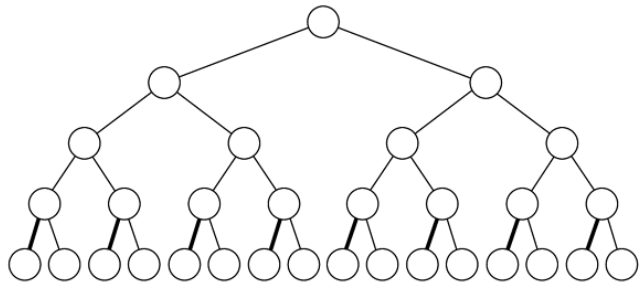
\includegraphics[width=0.5\textwidth,height=\textheight]{images/6.png}
\caption{Marking the left edges for height 1 nodes}
\end{figure}

\begin{figure}
\centering
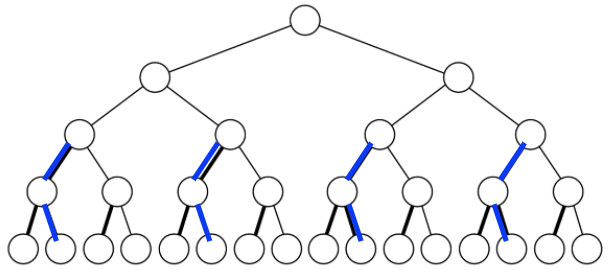
\includegraphics[width=0.5\textwidth,height=\textheight]{images/7.png}
\caption{Marking the first left edge and the subsequent right edge for
height 2 nodes}
\end{figure}

\begin{figure}
\centering
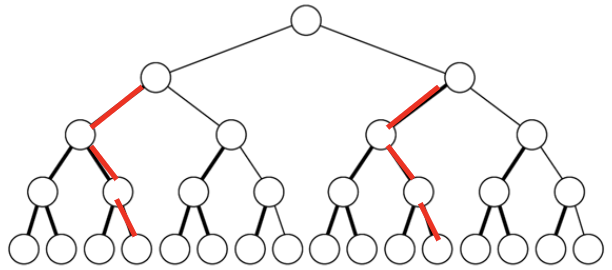
\includegraphics[width=0.5\textwidth,height=\textheight]{images/8.png}
\caption{Marking the first left edge and the subsequent two right edges
for height 3 nodes}
\end{figure}

\begin{figure}
\centering
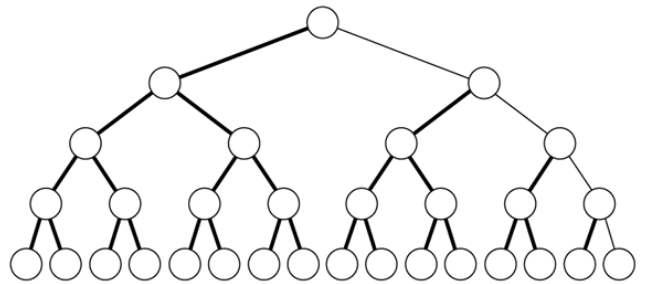
\includegraphics[width=0.5\textwidth,height=\textheight]{images/9.png}
\caption{Completed Marking}
\end{figure}

\begin{itemize}
\tightlist
\item
  After we're finished darkening all the nodes, the rightmost path is
  still not marked

  \begin{itemize}
  \tightlist
  \item
    There are \(h\) edges in that path
  \item
    The total number of edges is \(n-1\)
  \item
    The total number of edges marked is \(n-h-1\)
  \end{itemize}
\end{itemize}

\hypertarget{heap-sort-summary}{%
\subsection{Heap Sort Summary}\label{heap-sort-summary}}

\begin{itemize}
\tightlist
\item
  Time complexity

  \begin{itemize}
  \tightlist
  \item
    \(O(n\log(n))\)
  \end{itemize}
\item
  Space complexity

  \begin{itemize}
  \tightlist
  \item
    Delete and put it into a second array: \(O(n)\) additional memory
  \item
    Delete only at the end of the array: no extra memory involved
  \end{itemize}
\item
  Stable?

  \begin{itemize}
  \tightlist
  \item
    A \emph{stable sort} maintains order among equal items. An example
    of sorting the following items: \(1_a, 2, 1_b\)

    \begin{itemize}
    \tightlist
    \item
      Stable sort: \(1_a, 1_b, 2\)
    \item
      Unstable sort: \(1_a, 1_b, 2\) or \(1_b, 1_a, 2\)
    \end{itemize}
  \end{itemize}
\end{itemize}

\hypertarget{next-lecture}{%
\subsection{Next Lecture}\label{next-lecture}}

\begin{itemize}
\tightlist
\item
  Topic: Balanced Binary Search Trees

  \begin{itemize}
  \tightlist
  \item
    Reading: Chapter 19
  \end{itemize}
\end{itemize}

\end{document}
